\documentclass[DM,lsstdraft,toc]{lsstdoc}
\usepackage{graphicx}
\usepackage{url}
\usepackage{latexsym}
\usepackage{color}
% black, blue, brown, cyan, darkgray, gray, green, lightgray, lime, magenta, blue, orange, pink, purple, red, teal, violet, white, yellow.
\usepackage{enumitem}
\usepackage{esvect}

\title[Detection Efficiencies]{Characterizing {\tt DIASource} Detection Efficiency}

\author{M.~L.~Graham et al., and the DM SST}

\setDocRef{DMTN-TBD}
\date{\today}
\setDocUpstreamLocation{\url{https://github.com/lsst-dm/dmtn-tbd}}


% % % % % % % % % % % % % % % % % %
\setDocAbstract{The goals of this study are to: (1) validate that the planned DM data products which characterize {\tt DIASource} detectability will meet the scientific needs of the community; (2) ensure that the requirements related to the characterization of {\tt DIASource} detectability are adequately flowed down, and that DM's plans are accurately expressed in the DM documentation; and (3) inform the community about the planned DM data products related to {\tt DIASource} detectability.}


\setDocChangeRecord{%
\addtohist{0.0}{2018-11-01}{Internal working document.}{Melissa Graham}
\addtohist{0.1}{2019-09-09}{Updated to represent DM's plans.}{Melissa Graham}
\addtohist{1}{2022-04-dd}{Update and release.}{Melissa Graham}
}

\begin{document}

\maketitle

% CITATION EXAMPLES
% \verb|\citellp|: \citellp{LPM-17, LSE-30} \\
% \verb|\citell|: (SRD; \citell{LPM-17,LSE-29}) \\
% \verb|\citep[][]|: \citep[e.g.,][are interesting]{LPM-17,LSE-29} \\
% \verb|\cite|: \cite{LPM-17,LSE-29}
% \citeds{LSE-163}, \citedsp{LSE-163}


% % % % % % % % % % % % % % % % % %
\section{Introduction} \label{sec:intro}

Any astrophysical question which asks, e.g., {\it "How often?"} or {\it "How many?"} about transient phenomena, such as population studies or occurrence rates, needs to know a survey's {\it detection efficiency}: the probability that a source is detected (or in other words, the fraction of all sources that are detected).

Detection efficiencies are required for many of the core science pillars of the LSST, such as transient phenomena, cosmology, and Solar System studies  (Appendix~\ref{sec:sci}).
Many other surveys use populations of synthetic sources injected into the data in order to characterize the detection efficiency (Appendix~\ref{ssec:sci_trans}).

Rubin Observatory documentation contains no requirements related to producing or serving detection efficiencies for transient {\tt DIASources} in difference images (Appendix~\ref{sec:docs}), but does contain requirements about creating source injection software and using it to characterize detected sources' {\it spuriousness} parameter (see Appendix~\ref{sec:rb}).

As described in Appendix~\ref{sec:opts}, leaving synthetic source injection and the derivation of LSST detection efficiencies for transients as a user-generated data product is a moderate risk to LSST science.

This risk could be mitigated with a bit of extra effort on behalf of Data Management (and/or the Rubin Data Production team in Operations) to (1) ensure the artificial sources injected in order to characterize spuriousness cover the range of parameters needed to determine detection efficiencies, and (2) generate and provide a table of detection efficiencies.

The range of parameters that should be covered, and an example use-case of the table of detection efficiencies, is provided in Section~\ref{sec:proposal}. 

Readers should refer to the Data Products Definitions Document \citedsp{LSE-163} for more information about DIA, difference images, and {\tt DIASources}.
Detection efficiencies of extended difference-image sources (e.g., light echoes, trailed moving objects), or for variable or static point-sources in direct images, are beyond the scope of this document.


% % % % % % % % % % % % % % % % % %
\clearpage
\section{Proposed Detection Efficiency Matrix}\label{sec:proposal}

{\bf Detection:} as described in the SRD and DPDD, sources in difference images with a signal-to-noise ratio $SNR > {transSNR} = 5$ will be considered {\it detected} and will become a {\tt DIASource}.
 
{\bf Detection Efficiency:} The probability that a true astrophysical source of a given magnitude is detected and becomes a {\tt DIASource}. In other words, the fraction of all true astrophysical sources of a given magnitude that are detected and become {\tt DIASources}. 

Characterizing detection efficiency requires knowing how many sources were in the field of the image (and their brightnesses), which is only be possible if ``truth" is somehow known from, e.g., co-temporal imaging data of superior quality -- which almost never exists because it is inefficient to duplicate data.

Instead, the detection efficiency is typically characterized by simulating and injecting synthetic sources into images, using a point-spread function shape like real astrophysical sources, and then processing the images with the survey's difference image analysis pipeline and measuring the fraction recovered.

The detection efficiency can be characterized as $\eta(m)$, where $m$ is the apparent magnitude of the time-changing component with respect to the template image, and $\eta$ is a value between $0$ and $1$ that represents the probability that the source would be detected in the difference image.
As described in Appendix~\ref{sec:sci}, $\eta$ depends on more than just $m$, and is a function of the parameters ($\vv{P}$) listed in Table \ref{tab:eta_pars}.

An accurate measure of $\eta(m,\vv{P})$ for every pixel of every difference image is technologically unfeasible.
Instead, an analytic model for $\eta(m,\vv{P})$ can be built, so long as the synthetic sources cover the full range of $m$ and $\vv{P}$.

As described in Appendix~\ref{sec:sci}, for $\eta(m,\vv{P})$ the synthetic sources do {\it not} need to accurately represent astrophysical transient types in terms of their colors, redshifts, host offsets, durations, light curves, etc.
That aspect of the analysis is best left to the user to handle for their particular type of object, as described in Section~\ref{sec:proposal}.

A specific example of how users might apply $\eta(m,\vv{P})$ in their analysis is provided in Appendix~\ref{ssec:sci_cfht}.
Generally, it would involve simulating a set of light curves for the object type of interest (e.g., normal $0.1<z<0.5$ Type Ia supernovae), and then using the detection efficiency table to evaluate the fraction that would be ``identified" in a given time-frame (where ``identified" might have specific criteria, such as a reliable photometric classification).
This is typically done as part of an MC analysis in order to marginalize over intrinsic distributions of, e.g., the brightness or host offsets of the object type of interest.

\begin{table}[h]
\begin{center}
\begin{footnotesize}
\caption[]{A description of the image and source parameters ($\vv{P}$) that can affect the detection efficiency ($\eta(m)$) of point sources in a difference image (per filter).}
\label{tab:eta_pars}
\setlength{\extrarowheight}{5pt}
\begin{tabular}{|p{3.1cm}|p{12cm}|}
\hline
{\bf Parameter} & {\bf Description} \\
\hline
%Apparent Magnitude & Typically, $\eta$ decreases for fainter objects (and brighter objects due to saturation). \\
%\hline
Surface Brightness & Typically, $\eta$ decreases for objects embedded in brighter host galaxies. \\
\hline
Static-Source Offset & Sometimes, $\eta$ decreases for objects that are near (i.e., overlap the point-spread function of) static sources (e.g., stars, galaxy cores, especially if cuspy in profile). \\
\hline
CCD Location & With some instruments, $\eta$ decreases near the CCD edges due to distortion. \\
\hline
Image FWHM & The value of $\eta$ can decrease for extreme FWHM differences from the template (i.e., very good or very poor seeing). \\
\hline
Image Airmass & LSST images will experience differential chromatic refraction which affects image subtraction \citedsp{DMTN-037}, and thus potentially also $\eta$. \\
\hline
Sky Brightness & Typically, $\eta$ decreases when the sky background is bright or has a strong gradient (e.g., during twilight, near the moon). \\
\hline
Sky Cloud Cover & Extinction will affect $\eta$ by degrading the image magnitude limit. \\
\hline
\end{tabular}
\end{footnotesize}
\end{center}
\end{table}



\clearpage
\bibliography{local,lsst,refs,books,refs_ads}

% % % % % % % % % % % % % % % % % %
\appendix

\clearpage
\section{Scientific Examples}\label{sec:sci}

% % % % % % % % % % % % % % % % 
\subsection{Summary}

Detection efficiencies are required for many of the core science pillars of the LSST, as described below.
Many other surveys use populations of synthetic sources injected into the data in order to characterize the detection efficiency, as described in the examples provided in \ref{ssec:sci_trans}.

In consideration of the scientific motivation for detection efficiencies, and what has worked for other surveys, two points are clear.

\begin{enumerate}

\item The population of synthetic sources injected in order to characterize the detection efficiency should have similar distributions as real astrophysical phenomena in terms of brightness and location (e.g., proximity to static-sky sources, field crowdedness, surface brightness), and the subset of images used should sample the distributions of, e.g., image quality (seeing), sky brightness, and airmass. 

\item The simulated fakes do not need to accurately represent astrophysical transient types, colors, redshifts, durations, light curves, etc., or be planted in sequential images in a correlated way to represent real light curves.
That aspect of the analysis is best left to the user to handle during the MC simulation stage for their particular type of object.

\end{enumerate}

% % % % % % % % % % % % % % % %
\subsection{Transients}\label{ssec:sci_trans}

Transient events such as stellar explosions (supernovae, kilonovae) and tidal disruption events (TDEs; stars destroyed by close passage to a supermassive black hole) occur once and do not repeat.
Since most transient progenitors are stars, they are most often found in high surface brightness environments (i.e., galaxies; their spatial distribution ``follows the light") and require difference imaging in order to be discovered, and thus detection efficiencies in order to characterize their occurrence rates.
For example, transient occurrence rates as a function of environment can constrain their progenitor star characteristics, which requires that detection biases be well known, as does understanding selection biases in transient samples (e.g., when using Type Ia supernova as cosmological standard candles). 

The four surveys mentioned below have either inserted fakes into all of their live images (SDSS-II and DES) or into a representative set of images at a later time (CFHT and PTF), to ensure that detection efficiencies can be determined for the full range of image parameters.
In all cases, the fakes were simulated with parameter distributions (e.g., brightness, location) that roughly mimic the real astrophysical objects of interest for each particular survey (mostly supernovae, for the above examples).
Typically, the MC method was then used to simulate light curves for the transient of interest, and then the derived detection efficiencies were applied.

The take-away message is that, for Rubin Observatory to best serve a broad section of the transient community, the simulated population of fake sources need only be representative of true astrophysical sources in a bulk sense, in terms of their brightness and location (i.e., plant more faint sources than bright, and more in high surface-brightness areas than isolated regions).
The simulated fakes do not need to accurately represent astrophysical transient types, colors, redshifts, durations, light curves, etc., or be planted in sequential images in a correlated way to represent real light curves.
That aspect of the analysis is best left to the user to handle during the MC simulation stage for their particular transient type. 

\subsubsection{Sloan Digital Sky Survey II (SDSS-II)}

In order to calculate the occurrence rates of Type Ia supernovae (SNe\,Ia) from the SDSS-II, \cite{2008AJ....135..348S} generated a realistic sample of SNe\,Ia and injected fake point sources into the images as part of the live data processing pipeline to discover SNe\,Ia.
Additional simulations to evaluate on how often the fakes were recovered by the end-to-end SN\,Ia discovery pipeline were then required to evaluate how assumptions about the simulated population (e.g., the distribution of light curve stretches) contributed to the final uncertainty in the derived rates \citep{2008ApJ...682..262D}.
The final form of their derived detection efficiency for SNe\,Ia was $\epsilon(z) = (0.78 \pm 0.01) + (-0.13 \pm 0.14)z$, within which is captured assumptions about the true relative fraction of each SN\,Ia subtype, such as the under/over-luminous 91bg/91T-likes \citep{2008ApJ...682..262D}.
The detection efficiency, $\epsilon$, contributed to the final volumetric rate, $r_V = N / \widetilde{VT\epsilon}$, where $N$ is the number of SNe\,Ia detected, and $\widetilde{VT\epsilon}$ is the product of the effective survey volume, time, and detection efficiency.

\subsubsection{Dark Energy Survey (DES)}

In order to determine the SN\,Ia detection efficiency as a function of redshift, the DES team used a method very similar to SDSS-II: fake sources were injected into their live data, which was run through their real-time {\tt DiffImg} pipeline used to detect transients \cite{2015AJ....150..172K}.
This process also started by simulating a realistic sample of SNe\,Ia, with parameters such as light curve stretch, host offset, and subtype drawn from established underlying distributions, and then used a Monte Carlo simulation of many more SN light curves, combined with the detection efficiencies for their fakes, to determine the SN\,Ia detection efficiency as a function of redshift.
% The DES real/bogus algorithm an pipeline are described by Goldstein et al. 2015:
% http://adsabs.harvard.edu/abs/2015AJ....150...82G

\subsubsection{A Canada-France-Hawaii Telescope (CFHT) Cluster Survey}

In order to calculate the occurrence rate of SNe\,Ia in galaxy clusters for a CFHT imaging survey, \cite{2012ApJ...746..163S} performed DIA to detect SNe in real time, but the fake injection was done separately.
Simulated point sources were implanted into a representative subset of their images, and detection efficiencies calculated as a function of the relevant parameters for this survey: apparent magnitude, image quality, and focal plane location (because because the survey used single pointings with only small dithers).
Their expression for the rate of Type Ia supernovae per unit stellar mass is $R_{\rm Ia} = (N_{\rm Ia} / C_{\rm spec}) / ( \sum_{j=1}^{j=N_{\rm img}} \Delta t_j Mj )$, where $N_{\rm Ia}$ is the number of SNe\,Ia discovered in the survey, $C_{\rm spec}$ is the spectroscopic confirmation rate (determined separately), the denominator's sum is over all images of the survey, $M_j$ is the total stellar mass within the image, and $\Delta t_j$ is the control time for SNe\,Ia of that image.
The control time is expressed as $\Delta t = \int_{t_1}^{t_2} \eta(m(t)) dt$, where $m(t)$ is a SN\,Ia light curve, $\eta$ is the detection efficiency, and the integration limits are the survey's temporal boundaries.

The Monte Carlo method was then used to calculate $R_{\rm Ia}$ for the survey many times while sampling over a realistic distribution of SN\,Ia light curve properties for $m(t)$ and the errors in $N_{\rm Ia}$, $M_j$, and $eta$.
During this MC, an {\it effective} detection efficiency was used, which accounts for the possibility that the simulated SN\,Ia was detected in the previous two images: $\eta = \eta_j - \eta_j \eta_{(j-1)} - \eta_j \eta_{(j-2)} - \eta_j \eta_{(j-1)} \eta_{(j-2)}$ (as was appropriate for this surveys monthly cadence).
The final result was quoted as the median of the MC rates with $1\sigma$ errors. A similar methodology was applied to this survey's cluster SNe\,II in \cite{2012ApJ...753...68G}.

\subsubsection{Palomar Transient Factory (PTF)}

The PTF covered $8000$ square degrees with a three-to-five day cadence and generated over $1$ $\rm PB$ of data.
As detailed by \cite{2017ApJS..230....4F}, inserting fake sources into all of these images was both impractical and unnecessary.
Instead, they chose a single representative {\it field} and planted fake sources in all images of that field.
The fakes were given a uniform distribution in apparent magnitude, distributed in each image such that most of them are located within a galaxy, and then the PTF detection efficiencies were determined as a function of the apparent magnitude, the local surface brightness, and image parameters such as FWHM, airmass, moon illumination fraction, and sky background.
These detection efficiencies were used to derive the volumetric rate of normal SNe\,Ia \citep{2019MNRAS.tmp..772F}, of Ca-rich transients by \cite{2018ApJ...858...50F}, and of tidal disruption events (TDEs) by \cite{2018ApJS..238...15H}.
However, note that some rates analyses for TDEs have used aperture photometry and not difference imaging, and thus did not need fake injection for difference-image detection efficiencies (e.g., \cite{2016MNRAS.455.2918H}).

% Frohmaier uses stars from the field, not a simulated PSF: "clone-stamping".
% Frohmaier 2019 details: r_v(z) = (1/V deltaT) sum_{i=1}^N (1+z_i) / epsilon_i
% r_v(z) = volumetric rate of SNeIa at redshift z
% V = volume
% delta T = survey time
% sum over the number of SNeIa in the final sample
% (1+z_i) = cosmological time dilation factor
% epsilon_i = "detection efficiencies of each object"
% but note that epsilon != eta, rather epsilon is built from eta
% a large sample of SNeIa with realistic intrinsic properties are simulated, planted in the data, and then recovered, and then a grid of recovery fractions as a function of SNIa intrinsic properties and redshift is created, and those are the epsilons assigned to detected SNeIa


% % % % % % % % % % % % % % % %
\subsection{Cosmology}\label{ssec:sci_cosmo}

The selection function for Type Ia supernovae that are used in dark energy analyses must be well constrained.


% % % % % % % % % % % % % % % %
\subsection{Active Galactic Nuclei}\label{ssec:sci_agn}

Active Galactic Nuclei (AGN) are powered by a supermassive black hole in the center of a galaxy, surrounded by a gas disk.
Their energy output is non-thermal emission from X-ray through to mid-infrared, including emission lines in the optical spectrum, and many (or most) AGN exhibit optical variability.
As such, they appear as a variable point source in the cores of galaxies.
Many studies of AGN use aperture photometry on direct images, and not difference imaging, because it is desirable to have the {\it entire} flux of the AGN's point source, not just the flux in its variable component.

% The first to use variability to select AGN was Sarajedini et al. 2003; an two-epoch HST survey.
AGN samples have typically identified using spectroscopic emission lines, optical colors, or by looking for excesses of radio, X-ray, or mid-infrared emission, but selection by optical variability is also an option and in particular it may be better at including low-luminosity AGN, as described by \cite[e.g.,][]{2008A&A...488...73T,2010ApJ...723..737V}.
The detection method of \cite{2008A&A...488...73T} uses image subtraction for the initial detection of AGN candidates, mainly because difference imaging was already done to find supernovae in the survey.
Aperture photometry is then performed on the candidates, and a variability threshold applied to form their final sample for spectroscopic follow-up.
\cite{2010ApJ...723..737V} skip the difference imaging step and use aperture photometry and a statistical analysis true variability to identify AGN.
Neither use the injection of fake point sources to evaluate their detection efficiencies, and instead use objects with spectra and/or X-ray detections to estimate their completeness.
% De Cicco et al. 2015 is very similar to Trevese, done in the VST-SUDARE/VOICE survey for SNe.
However, using spectra or X-ray to characterize the sample selection function of AGN identified by optical variability might not be possible in the LSST era, when optical variability becomes a more efficient and prolific way to discover a AGN \cite[e.g.,][]{2014ApJ...782...37C}, generating significantly larger, lower-luminosity, and/or higher-redshift samples, for which spectroscopic confirmation is more difficult.

Furthermore, TDE and SNe also occur in the cores of galaxies \citep[e.g.,][]{2009A&A...507L..17P,2012ApJ...744L..19K}, causing contamination of the AGN samples, and quantifying the rate of missed transients in the cores of galaxies remains an open problem.

Considering the needs of the AGN, TDE, and SN communities suggests that a population of fake injected transients to characterize the difference-image detection efficiency of point sources in galaxy cores would be scientifically beneficial.



% % % % % % % % % % % % % % % %
\subsection{Variable Stars}\label{ssec:sci_varstar}

A star's luminosity might exhibit intrinsic variability (e.g., RR Lyrae, Cepheids) and/or extrinsic variability (e.g., eclipsing binaries, exoplanet transits, or microlensing events).
In uncrowded fields, using direct images and the total flux is preferable to difference-imaging analysis for scientific studies that aim to identify and characterize variable stars.
However, in crowded fields such as the Galactic plane, identifying variable stars in difference images can be much easier because the difference image is not as (or not at all) crowded, compared to the direct image.

For example, the census of variable stars in crowded fields by \cite{2016A&A...588A.128F} describes how difference imaging is used, although it does not appear that injecting fake sources or deriving detection efficiencies was needed for their analysis.

It also seems that difference-image detection efficiencies are not needed for microlensing studies, for which it is a common methodology to fit a PSF to every pixel of a difference image, concoct a "light curve", and then statistically assess whether it is consistent with the expected shape of a microlensing event \cite{2015ApJ...806..161L}\footnote{Although \cite{2015ApJ...806..161L} does mention that detection efficiencies would be used in a paper in preparation.}. 

Despite difference-image detection efficiencies not playing a role in past variable star studies, they might still be needed for LSST analyses.
For example, injecting new fake sources in crowded stellar fields might be useful for detection efficiencies for stars which are too faint to have a counterpart in the template, but whose variable component makes them detectable by LSST for a short while.
This would apply to e.g., M-dwarf flares (a common contaminant in searches for young SNe) and microlensing events.

Simulating variability of stars that {\it are} present in the template image is beyond the scope of this document.


% % % % % % % % % % % % % % % %
\subsection{Moving Objects}\label{ssec:sci_move}

All of the moving objects identified by LSST will first be detected as difference-image sources, and detection efficiencies would be useful for population studies.
In epochs of non-detection, being able to obtain the detection efficiency at a predicted location (i.e., as a function of local surface brightness and image qualities) would be a useful quantity for science goals related to moving object populations.
The probability of, e.g., a faint asteroid's chance alignment over bright galaxies is small, and so fake injected point sources in empty locations may be more useful for moving object science --- these would be needed to simulate very high-redshift transients, as well.

A consideration of whether the injection of trailed sources is scientifically useful is left for other work.



\clearpage
\section{Requirements Review}\label{sec:docs}

% % % % % % % % % % % % % % % % 
\subsection{Summary}

There are no requirements related to producing or serving detection efficiencies for transient {\tt DIASources} in difference images.

However, the OSS specifies that spuriousness characterization be done {\it ``by insertion and recovery of artificial sources"}, and the DMSR specifies that {\it software} for fake injection is a deliverable of the DMS (\S~\ref{ssec:docs_dmsr}).

This suggests that use of artificial source injection to determine a detection efficiency matrix for transient {\tt DIASources} would not require a large expansion of scope for DM.

As a final note, the DMS computational system is sized to accommodate the (re)processing of all images with fake sources implanted {\bf (from KT)}.

% % % % % % % % % % % % % % % % 
\subsection{Science Requirements Document (SRD, LPM-17)}

The SRD \citedsp{LPM-17}, V5.2.4 (Jan 30 2018), does not contain any requirements related to detection efficiencies.

The SRD does describe how the Prompt pipeline should provide {\it ``the fast release of data on likely optical transients will include measurements of position, flux, size and shape, using appropriate weighting functions, for all the objects detected above {\tt transSNR} signal-to-noise ratio in difference images"}, where {\tt transSNR} = 5 (page 41).

The SRD thus specifies that all sources with $SNR \geq 5$ in a difference image are considered ``detected", and it is the efficiency (or completeness) of detected transients (i.e., new sources which were not present in the template) that this document is concerned with.

% % % % % % % % % % % % % % % % 
\subsection{LSST System Requirements Document (LSE-29)}

The LSST \citedsp{LSE-29}, V7.1 (Mar 5 2020), does not contain any requirements related to detection efficiencies.


% % % % % % % % % % % % % % % % 
\subsection{Observatory System Specifications (OSS, LSE-30)}\label{ssec:docs_oss}

The OSS \citedsp{LSE-30}, V19.1 (July 30 2021) does not contain any requirements related to the determination of detection efficiencies.

However, it does contain several specifications related to characterizing the spuriousness (also referred to as the ``real/bogus" parameter), completeness, and purity of LSST sources detected in difference images.
See Appendix~\ref{sec:rb} for a description of these terms.

The "insertion and recovery of artificial sources" that are mentioned as a means towards achieving requirements 0351, 0353, and 0354 could also be used to determine detection efficiencies.

\begin{itemize}

\item OSS-REQ-0351\ossreq{0351}, {\it Difference Source Spurious Probability Metric}, specifies that {\it ``the Observatory shall develop a metric to characterize the probability of each reported difference source being spurious"} (Section 3.1.5.2.1.7.5).
The discussion further clarifies that {\it ``the performance of this metric will be assessed by simulations, by insertion and recovery of artificial sources, and comparisons to ground truth where known"}.

\item OSS-REQ-0352\ossreq{0352}, {\it Difference Source Sample Completeness}, specifies that {\it ``for each visit, the Observatory shall estimate the detected difference source sample completeness and purity as a function of the spuriousness metric threshold cut"} (Section 3.1.5.2.1.7.6).
The discussion further clarifies that {\it ``this information will aid the end
users in selecting the spuriousness threshold appropriate for their particular science case"}.

\item OSS-REQ-0353\ossreq{0353}, {\it Difference Source Spuriousness Threshold - Transients}, specifies that {\it ``there shall exist a spuriousness threshold {\tt T} for which the completeness and purity of selected difference sources are higher than {\tt transCompletenessMin} (90\%)\reqparam{transCompletenessMin} and {\tt transPurityMin} (95\%)\reqparam{transPurityMin}, respectively, at the SNR detection threshold {\tt transSampleSNR} (6)\reqparam{transSampleSNR}. This requirement is to be interpreted as an average over the entire survey"} (Section 3.1.5.2.1.7.7).
As for OSS-REQ-0351, the discussion further clarifies that {\it ``the performance of this metric will be assessed by simulations, by insertion and recovery of artificial sources, and comparisons to ground truth where known"}.

\item OSS-REQ-0354\ossreq{0354}, is similar to OSS-REQ-0353 but defines a threshold for moving objects.

\end{itemize}

Regarding spuriousness, the discussion for OSS-REQ-0351 further describes that the {\it ``spuriousness metric be prior free to the extent possible. For example, while it may make use of information from the source and image characterization (e.g., comparison of source to PSF morphology), as well as the information on the Telescope and Camera system (e.g., ghost maps, defect maps, etc.), it will not use any information about the astrophysical neighborhood of the source, whether it has been previously observed or not, etc. The intent is to avoid introducing a bias against unusual sources or sources discovered in unusual environments"}.


% % % % % % % % % % % % % % % % 
\subsection{Data Management System Requirements (DMSR, LSE-61)}\label{ssec:docs_dmsr}

The DMSR \citedsp{LSE-61}, V9.0 (Feb 12 2021) does contain a few statements relevant to detection efficiencies. 

\begin{itemize}

\item DMS-REQ-0097\dmreq{0097}, {\it "Level 1 Data Quality Report Definition"}, specifies that the Data Management System (DMS) {\it ``shall produce ... indicators of data quality that result from running the DMS pipelines, including ... detection efficiency for point sources vs. mag for each utilized filter"} (Section 1.3.14).
However, DMS-REQ-0097 is derived from OSS-REQ-0131, {\it ``Nightly Summary Products"}, and is clearly intended to produce a nightly summary of the general performance of the observatory and the DMS, not to provide the scientifically useful detection efficiencies that are the topic of this document. 

\item DMS-REQ-0009\dmreq{0009}, {\it ``Simulated Data"}, specifies that {\it ``the DMS shall provide the ability to inject artificial or simulated data into data products to assess the functional and temporal performance of the production processing software"} (Section 3.2.1).
This requirement is derived in part from OSS requirements 0351, 0353, and 0354 discussed above.

\end{itemize}


% % % % % % % % % % % % % % % % 
\subsection{Data Products Definitions Document (DPDD, LSE-163)}\label{ssec:docs_dpdd}

The DPDD \citedsp{LSE-163}, V3.6 (Dec 17 2021) is not a requirements document but does have some information relevant to detection efficiencies.

Table 1 lists a single float is also reserved for ${SNR}$ in the DPDD's {\tt DIASource} table, defined as the {\it ``signal-to-noise ratio at which this source was detected in the difference image"}.

Table 1 also lists a single float is reserved in the {\tt DIASource} table for the spuriousness parameter.
The DPDD's definition and description of spuriousness match the OSS requirement (i.e., this is a direct flow-down of OSS-REQ-0351\ossreq{0351}).

The {\tt DIASource} catalog table has three other relevant parameters listed that might be scientifically useful for analyses involving detection efficiencies:
\begin{itemize}
\item {\tt psLnL [float]} -- {\it Natural log likelihood of the observed data given the point source model.} This represents the probability that a detected source is a point source; detection efficiencies would not apply to non-point sources.
\item {\tt fpBkgd [float]} $\rm nJy/asec^2$ -- {\it Estimated background at the position (centroid) of the object in the template image.} This will be useful to provide detection efficiencies in difference images as a function of the background at that location.
\item {\tt fpBkgdErr [float]} $\rm nJy/asec^2$ -- {\it Estimated uncertainty of {\tt fpBkgd}.} Useful in the same way as {\tt fpBkgd}. 
\end{itemize}


% % % % % % % % % % % % % % % % 
\subsection{Data Management Science Pipelines Design (LDM-151)}\label{ssec:docs_ldm151}

\citeds{LDM-151}, V4.3 (Nov 10 2020), details the scientific design and implementation of the requirements set by the SRD, OSS, and DMSR, and the generation of the data products described in the DPDD.

Section 3, {\it ``Alert Production"}, states that {\it ``In this document we do not address estimation of the selection function for alert generation through the injection of simulated sources. Such a process could be undertaken in batch mode as part of the DRP."}

However, \citeds{LDM-151} does make two relevant statements about the {\tt spuriousness} parameter which describe how the real-bogus algorithm will likely {\it ``be based on a trained random forest classifier ... conditioned on the image quality and airmass"} (Section 3.2.4) and that it  {\it ``may use machine learning on other measurements or pixels"} (Section 6.7.2).


%Section 3.2.4, {\it ``Difference Imaging"}, states that {\it ``The application of spuriousness algorithms, also known as 'real-bogus', may be applied at this time dependent on whether the number of false positives is less than 50\% of the detected sources. ... The default technique will be based on a trained random forest classifier. It is likely that the training of this classifier will need to be conditioned on the image quality and airmass of the observations."} 

% Section 6.7.2, {\it ``Algorithms"}, states that the {\tt spuriousness} measurement is a {\it ``per-source measure of likelihood the detection is junk (in a difference image)"} that {\it ``may use machine learning on other measurements or pixels"} and {\it ``may be augmented by spuriousness measures that aren't purely per-source"}. Figure 12, a matrix showing the algorithms applied to the different types of measurements (single visit, difference image, etc.) shows that a different implementation or algorithm for {\tt spuriousness} will be used for the Difference Image Measurement compared to the Single Visit, Multi-Coadd, Multi-Epoch, and Forced Measurements.

% Section 5.6.3, {\tt MakeSelectionMaps}, states that this calibration step {\it ``is responsible for producing multi-scale maps that describe LSST's depth and efficiency at detecting different classes of object. The details of what metrics will be mapped, the format and scale of the maps (e.g. hierarchical pixelizations vs. polygons), and the way the metrics will be computed are all unknown".} It also states that this must be extendable to Level 3, but that {\it ``the details of what DM will provide still needs to be clarified to the community"}, and notes that the reprocessing time for fake plants could be prohibitive. However, this referring to the depth and efficiency of detecting static-sky objects in the direct images or deep coadds, not transients/variables in the difference images.



\clearpage
\section{Spuriousness (Real/Bogus)}\label{sec:rb}

The completeness, purity, and spuriousness of samples of detected sources are all related to detection efficiencies. 

When source detection is performed on a difference image, both true astrophysical sources and artifact sources can be detected with $SNR > {transSNR} = 5$ and become {\tt DIASources}.
Examples of artifacts include, e.g., sources caused by telescope hardware, or incompletely removed cosmic rays (despite the fact that cosmic rays are real astrophysical messengers). 

{\bf Spuriousness ($\mathcal{S}$):} a parameter, typically between $0$ and $1$, which represents the probability that a source is astrophysical (values closer to $1$) or artifact (values closer to $0$).

The spuriousness is sometimes also called the {\it real/bogus score}.
It is typically determined by machine learning on many sources that were pre-classified as astrophysical (real) or artifact (bogus), and usually considers factors like the shape of the point source in the difference image (e.g., symmetry, sharpness). 

{\bf Spuriousness Threshold ($\tau_{\mathcal{S}}$):} a lower limit on spuriousness, $\mathcal{S}$, which can be applied to {\tt DIASources} to separate the "real" from the "bogus", and to thereby obtain a subset of {\tt DIASources} with a lower fraction of artifacts. 

The following definitions describe the classification of detected {\tt DIASources}, which were either truly real (astrophysical source) or truly false (artifact), as real or bogus by an applied spuriousness threshold $\tau_{\mathcal{S}}$:

\begin{tabular}{rl}
True Positive ($\mathit{TP}$) & A detected astrophysical source that was classified as real. \\
False Positive ($\mathit{FP}$) & A detected artifact that was classified as real. \\
True Negative ($\mathit{TN}$) & A detected artifact that was classified as bogus. \\
False Negative ($\mathit{FN}$) & A detected astrophysical source that was classified as bogus. \\
\end{tabular}

{\bf Completeness ($\mathcal{C}$):} the fraction of all detected astrophysical sources which are classified as real. This is also called the true positive rate, $\mathit{TPR} = \frac{\mathit{TP}}{\mathit{TP}+\mathit{FN}}$.

{\bf Purity ($\mathcal{P}$):} the fraction of all detected sources that were classified as real which are astrophysical in nature: $\frac{\mathit{TP}}{\mathit{TP}+\mathit{FP}}$. This is also called the {\it precision} or the {\it positive predictive value} ($\mathit{PPV}$) of a survey. 

The false positive rate\footnote{Note that in some published literature the false positive rate is instead defined as the fraction of all detected artifacts that were classified as real, $\mathit{FPR} = \frac{\mathit{FP}}{\mathit{TN}+\mathit{FP}}$.} is the fraction of all detected sources that were classified as real but which are artifacts: $\mathit{FPR} = 1 - \mathit{PPV} = \frac{\mathit{FP}}{\mathit{TP}+\mathit{FP}}$.

The relationship between the completeness and purity of a sample of {\tt DIASources} classified as real can be traced out by varying $\tau_{\mathcal{S}}$.

In Figure \ref{fig:comp_pure} we show, as an example, the relationship between the false positive rate ($\mathit{FPR}$; purity) and the missed detection rate ($\mathit{MDR}$; completeness) for different types of source classification (i.e., real/bogus) algorithms from the Palomar Transient Factory \citep[PTF;][]{2013MNRAS.435.1047B}.
This relationship is formally known as the Receiver Operating Characteristic (ROC) curve when it is plotted as the true positive rate {\it vs.} the false positive rate for a given {\tt transSNR}.

\begin{figure}
\begin{center}
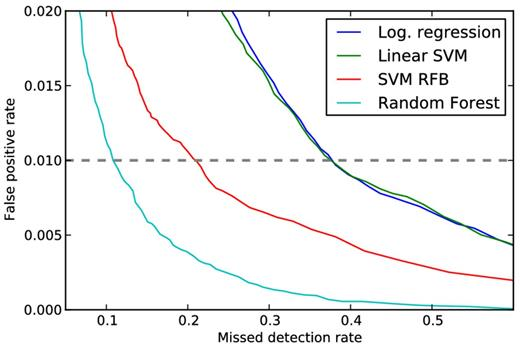
\includegraphics[width=8cm,trim={0cm 0cm 0cm 0cm}, clip]{figures/Brink_etal_2013_Fig3.jpg}
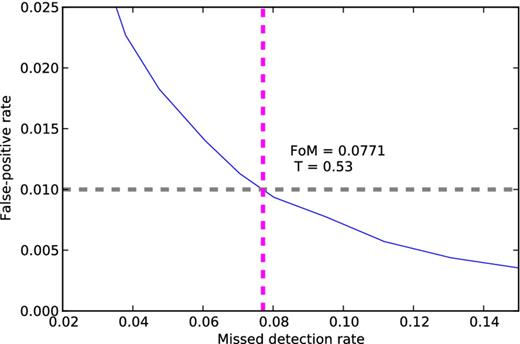
\includegraphics[width=8cm,trim={0cm 0cm 0cm 0cm}, clip]{figures/Brink_etal_2013_Fig7.jpg}
\caption{{\it Left:} An example of the relationship between the false positive rate ($\mathit{FPR}$; purity) {\it vs.} the missed detection rate ($\mathit{MDR}$; completeness) for different types of source classification (real/bogus) algorithms considered by the Palomar Transient Factory \citep{2013MNRAS.435.1047B}. {\it Right:} The relationship between $\mathit{FPR}$ and $\mathit{MDR}$ for the RB2 (real-bogus version 2) classifier (blue line) developed by the PTF and introduced in \cite{2013MNRAS.435.1047B}. Dashed lines show how $\mathit{FPR}=0.01$ is achieved with a spuriousness (real-bogus score value) threshold of $\tau=0.53$, which results in $\mathit{MDR}=0.077$. \label{fig:comp_pure}}
\end{center}
\end{figure}

{\bf Characterizing spuriousness} requires knowing which of the detected {\tt DIASources} are astrophysical (truly real) and which are artifacts (truly bogus).
Synthetic source injection is best for simulating astrophysical (real) sources because artifacts (bogus) can be a very diverse group; source injection cannot reveal which {\tt DIASources} in an image are artifacts.
Instead, characterizing spuriousness is achieved by building a training set of point sources that have been confirmed as astrophysical and artifact, using that training set for the spuriousness ($\mathcal{S}$; real/bogus) assignments by the machine learning algorithm.
Then, since ${transSNR}\propto m$, the ROC curve yields $\mathcal{C}(m,\tau_{\mathcal{S}})$ and $\mathcal{P}(m,\tau_{\mathcal{S}})$.


\clearpage
\section{Options Regarding Detection Efficiencies} \label{sec:opts}

The options for DM to participate in generating detection efficiencies, $\eta(\vv{P})$, are listed and discussed in terms of scope, risk, requirements, and science. 

% % % % % % % % % % % % % % % % 
\subsection{Do Nothing}\label{ssec:opts_no}

In this scenario, the data from any fake injection that is done in order to meet the requirement to characterize the spuriousness is not made available, but the science community would have access to the {\it software} for fake injection.

{\bf Scope --} No expansion of scope. \\
{\bf Risk --} A moderate risk in that multiple user groups may then need to perform fake injection, leading to redundant reprocessing of the data and a computational strain on the resources. \\
{\bf Requirements --} Does not violate or fulfill any requirements. \\
{\bf Science --} This option would negatively impact science results based on transient phenomena, one of the four pillars of LSST science. The need for computationally intensive processing would force multiple teams to compete, and might limit the number of individuals or teams who could successfully derive detection efficiencies, and thus limit the scientific applications.

% % % % % % % % % % % % % % % % 
\subsection{Make Available the Fakes Injected for Spuriousness Characterization}\label{ssec:opts_makefakeavail}

In this scenario, the data generated by the injection and recovery artificial sources in order to meet the requirements to characterize the spuriousness parameter is made available so that users may calculate detection efficiencies. For example, a {\tt DIASource}-like catalog for the fake injected point sources, which users could bin by the $\vv{P}$ relevant to their science and generate $\eta(\vv{P})$. Since the current OSS requirements are to characterize the relationship between $\tau_{\mathcal{S}}$ and sample completeness {\it only as a function of visit image qualities} for {\tt DIASources} with SNR$>$5 (\S~\ref{sec:docs}), this scenario does not guarantee that these artificial sources will be adequate for all science use-cases. 

{\bf Scope --} Possible expansion of scope to make available the fake-source catalogs. \\
{\bf Risk --} Minor risk, if the fake sources do not adequately cover $\vv{P}$, for the same reason as in \S~\ref{ssec:opts_no}. \\
{\bf Requirements --} Does not violate or fulfill any requirements. \\
{\bf Science --} Allowing users to build detection efficiency matrices from the same fake sources as are used to characterize spuriousness would enable at least some scientific analyses.

% % % % % % % % % % % % % % % % 
\subsection{Ensure the Fakes Injected for Spuriousness Characterization Meet Science Goals}\label{ssec:opts_ensurefakeP}

This scenario is similar to that in \S~\ref{ssec:opts_makefakeavail}, except the fake sources that are injected and recovered in order to meet the requirements to characterize the spuriousness parameter are scientifically validated to cover the parameters needed for scientific analyses, $\vv{P}$, as listed in Table \ref{tab:eta_pars}.

{\bf Scope --} Minor expansion of scope to validate the artificial sources cover an adequate range of parameter space, $\vv{P}$, and to make available the fake-source catalogs. \\
{\bf Risk --} No risk. \\
{\bf Requirements --} Does not violate or fulfill any requirements. \\
{\bf Science --} Allowing users to build detection efficiency matrices from a scientifically-validated set of artificial sources would enable more scientific analyses.

% % % % % % % % % % % % % % % % 
\subsection{Generate and Provide Detection Efficiencies}\label{ssec:opts_deteffs}

This scenario takes that of \S~\ref{ssec:opts_ensurefakeP} one step further, and has the DMS generate and provide the detection efficiency matrix, $\eta(\vv{P})$, as a scientifically validated and verified data product.

{\bf Scope --} Moderate expansion of scope to generate $\eta(\vv{P})$. \\
{\bf Risk --} No risk. \\
{\bf Requirements --} Does not violate or fulfill any requirements. \\
{\bf Science --} Enables scientific analyses for all that need detection efficiencies.

% % % % % % % % % % % % % % % % 
%\subsection{Generate Detection Efficiencies Without Fake Injection}\label{ssec:opts_nofakes}
%\textcolor{red}{MLG: I've heard RL say there are other ways to generate detection efficiencies than fake injection, but outside of co-temporal data of superior quality (which will not be available), I'm not sure how to know how many real things are missed as a function of apparent magnitude and other parameters. Maybe RL can fill in this section.}

\subsection{Inject Fakes during Prompt or Data Release Processing?}\label{ssec:opts_fakeswhen}

Here is considered three possible points in the data processing where the fake injection could be performed: during Prompt processing (\S~\ref{sssec:opts_fakeswhen_PP}), on an intermediate timescale between Prompt and Data Release processing (\S~\ref{sssec:opts_fakeswhen_int}), and during DR processing (\S~\ref{sssec:opts_fakeswhen_DR}).

\subsubsection{During Prompt Processing}\label{sssec:opts_fakeswhen_PP}

Inject fake sources into the live data which is processed within 60 seconds of image readout ({\tt OTT1}). With this option, fake sources would be injected {\it on the fly into every new visit image from the telescope processed with DIA} (or into the template image as negatives). This may seem like an extreme option to propose, but as discussed in \S~\ref{ssec:sci_trans} some previous transient surveys have injected fakes into their real-time pipelines, so we consider it here as well. 

{\bf Scientific Motivation for Prompt Fakes --} Surveys that plant artificial sources into live data processing typically use realistic light curves that represent their target population (e.g., color, duration, and location), and inject the fakes into sequential images in order to simulate real transients. The objective of this level of real-time injection is usually not just to characterize the detection efficiency, but also biases in the survey's classification algorithms and/or follow-up programs. Simulating fake sources that represent {\it real transient light-curves} in sequential images and in different filters in a realistic way is {\it not} being proposed here. Furthermore, most of the scientific analyses that require detection efficiencies, such as occurrence rates and population studies, would be done with the DIA products from a data release, and not the prompt products. A continually-updated detection efficiency matrix, $\eta(\vv{P})$, that incorporates data from fakes injected during Prompt processing does not have a strong scientific motivation.

{\bf Interference with Astrophysical Sources -- } In this scenario, fake sources would be planted into new images in a manner that samples the range of parameters for $\eta(\vv{P})$. This process would be comprised of three steps: (1) identify coordinates where the fakes should be planted, (2) fake injection into the image, and (3) bookkeeping for the fakes to ensure they do not contaminate the Alert Stream or the {\tt DIASource} catalog. Fakes should not be injected at random locations because it is important to sample regions with higher surface brightness and to avoid the locations of known {\tt DIAObjects}. If 1000 fakes are  assigned random locations and injected into a 3.2 Gp image, and we assume that image has 10000 (randomly-distributed) true sources in it, then the probability that none of the fakes are coincident with one of the true sources is $0.9968$. However, over a full night of 1000 visits, the probability that none of the fakes ever landed on a true source in any image is $0.0437$, and it is most likely ($P=0.2218$) that 3 fakes would have interfered with true sources. 
% from scipy.stats import hypergeom
% import matplotlib.pyplot as plt
% [M,n,N] = [3200000000,10000,1000]
% rv = hypergeom(M,n,N)
% print( rv.pmf([0,1,2,3,4]) )
% [  9.96843454e-01   3.11521588e-03   4.86216368e-06   5.05362508e-09   3.93505558e-12]
% [M,n,N] = [3200000000000,10000000,1000000]
% rv = hypergeom(M,n,N)
% print( rv.pmf([0,1,2,3,4]) )
% [ 0.04367555  0.13880061  0.21497859  0.22180274  0.17274015]

{\bf Benefits and Drawbacks of Prompt Fakes from a DM Perspective -- } Two of the benefits (to LSST DM) of fake injection during Prompt processing are that (1) it would negate the need for separate re-processing of all fake-infused images, which could increase the total computational budget by up to a factor of $2$, and (2) it could offer real-time feedback on evolution in the survey's completeness or purity, which might be useful --- however, real-time feedback is not a necessary component of the DMS and could be obtained via the spuriousness parameters, as completeness and purity correlate mainly with bulk image properties. Two of the main drawbacks of planting fakes into "live" data are that (1) only a small number should be planted so as to minimize the risk of interference with real phenomena and (2) the additional steps of simulating, planting, and verifying fakes must be included in the computational budget for Prompt processing, which completes within $60$ seconds for every new direct image and is already tightly constrained. 

{\bf Scope --} An expansion of scope in terms of FTE work hours and computational resources. \\
{\bf Risk --} A risk to the DMS by adding three steps to the 60-second processing budget and potentially interfering with the completeness and purity of {\tt DIASources}. \\
{\bf Requirements --} Does not violate any requirements (and is not necessary to meet any requirements). \\
{\bf Science --} This option would provide scientifically useful detection efficiencies, however, it may compromise science results if it interferes with the completeness and purity of {\tt DIASources}. As there would be a limit on the number of fakes injected into every image, and restrictions that those fakes be away from most true transients and variables, this method would not provide the {\it best} characterization of the survey's detection efficiencies.

% % % % % % % % % % % % % % % % 
\subsubsection{On an Intermediate Timescale}\label{sssec:opts_fakeswhen_int}

As a compromise between injecting fakes during Prompt Processing (above) and during Data Release Processing (below), fakes could be injected and recovered on a intermediate timescale (e.g., daily, weekly, monthly). There would be no need to reprocess {\it every} image because the goal is to build up a detection efficiency model as a function of parameters like host background, seeing and airmass. This pipeline could include only images in the parameter space where additional fakes are required. However, as with the proposed option to do fake injection during Prompt processing, there is no science case (or internal use-case) that requires the detection efficiencies updated in real time.  

{\bf Scope --} An expansion of scope in terms of both FTE and computational resources of the DMS. \\
{\bf Risk --} A risk to the DMS (increasing the amount of processing done in between DRs). \\
{\bf Requirements --} Does not violate any requirements. \\
{\bf Science --} This option would enables rates analyses on the Prompt data products, but these analyses are more likely to be done on the DR data products anyway, so it is unlikely that this option opens the door for any new --- or otherwise inaccessible --- science. 

% % % % % % % % % % % % % % % % 
\subsubsection{During Data Release Processing}\label{sssec:opts_fakeswhen_DR}

The benefits of implanting artificial sources into images during the DIA which occurs as a part of the annual DR processing is that fakes can be injected (1) only in locations where there were no detected {\tt DIASources} and (2) in all images without increasing the total computational budget by any more than is required to inject the PSFs. As described in Section \ref{sec:docs}, it is likely that fake injection would be done as part of DIA during DR processing anyway, in order to characterize the spuriousness parameter. This option is only be adding a step to ensure that the fakes are injected in a way that samples the parameter space $\vv{P}$ (Table \ref{tab:eta_pars}), as needed to use the fakes for detection efficiencies. These DR-derived detection efficiencies could be used on the Prompt data products for the following year. 

{\bf Scope --} A mild expansion of scope in terms of FTE, but potentially not in terms of computational resources. \\
{\bf Risk --} No risks. \\
{\bf Requirements --} Does not violate any requirements. \\
{\bf Science --} Enables science with both the DR and Prompt data products. 


% % % % % % % % % % % % % % % % 
\subsection{Could Detection Efficiencies be Derived from Provided Data Products?}\label{ssec:docs_derDE}

Could the spuriousness parameter $\mathcal{S}$, and the relationship between $\tau_{\mathcal{S}}$ and completeness --- both of which are specified by the OSS to be included in the data products (\S~\ref{ssec:docs_oss}) -- be used to create a full detection efficiency matrix, $\eta(\vv{P})$? In other words, could the following process be used? (1) bin the {\tt DIASources} by $\vv{P}$; (2) calculate the mean spuriousness as a function of apparent magnitude in the bin ($\bar{\mathcal{S}}(m)$); (3) use the established relationship between $\tau_{\mathcal{S}}(m)$ and completeness (\S~\ref{ssec:docs_oss}) to derive $\eta(\vv{P})$.

No. First, the relation between $\tau_{\mathcal{S}}$ and completeness (\S~\ref{ssec:docs_oss}) provides the completeness for all sources with $\mathcal{S}>\tau_{\mathcal{S}}$, whereas the scientific analyses will want the completeness in discrete bins. Second, this relation has already marginalized over parameters $\vv{P}$, and to attempt to "reverse-engineer" them will not be accurate. Third, using the {\tt DIASources} to derive $\eta(\vv{P})$ will lead to a bias, since only {\it already detected} objects are contributing to the detection efficiency. 
% the current OSS requirements are to characterize the relationship between $\tau_{\mathcal{S}}$ and sample completeness {\it only as a function of visit image qualities} (\S~\ref{sec:docs}). 


% % % % % % % % % % % % % % % % 
\subsection{Summary of Options}\label{ssec:opts_sum}

It would be scientifically useful -- with only a potential small increase in scope, if any -- to ensure that the artificial sources implanted to characterize the {\tt DIASouce} spuriousness parameter sample the parameter space needed for scientific analyses involving detection efficiencies, $\vv{P}$ (e.g., Table \ref{tab:eta_pars}), and to make the data from the injection and recovery of fake sources available to users so that they can build detection efficiency matrices $\eta(\vv{P})$. It would be even more useful to provide $\eta(\vv{P})$ as a scientifically validated data product. For both scenarios, doing the fake injection during the DIA which occurs as a prt of the annual Data Release processing both achieves the science goals and minimizes scope increase and risk to the DMS.


\clearpage
\section{Options for Fake Point Source Injection Techniques}\label{sec:tech}

There are a variety of ways in which fake sources can be simulated and injected into the images. Some options are more suitable for transients (\S~\ref{ssec:tech_new}), and some for variable stars (\S~\ref{ssec:tech_pre}). The following is a precursory presentation of the options, some of which have been used in the science studies discussed in \S~\ref{sec:sci}. Typically, artificial sources -- positive or negative -- are added to the direct image {\it before} that image enters the difference imaging pipeline, so that the detection efficiency captures the end-to-end pipeline efficiency for detecting difference-image sources. (This is why fakes are not typically injected into the final difference image prior to source detection).

% % % % % % % % % % % % % % % % 
\subsection{Simulating New Fake Objects}\label{ssec:tech_new}

This applies to point sources that appear where there was no point source in the template image, such as transients like supernovae, variable stars that are undetectable in their quiescent state, and moving objects (assuming they're slow-moving enough to not appear as trailed sources, which is a different problem not included in this study). 

Artificial sources that represent new fake objects would be planted in and around galaxies in a way that samples the environments of known transients (and serves the use-cases of variable stars and moving objects projected on background galaxies), would adequately sample areas of open space where most moving objects, some variable stars, and high-$z$ transients with undetectable hosts will be found, and also in crowded fields where many variable stars will be discovered.

{\bf Model PSF ---} A 2D model for the PSF is added to the direct image in order to simulate a new point source. The shape of the PSF is derived from known trends with, e.g., the focal plane location or airmass (DCR), and the brighter/fatter effect.

{\bf Clone-Stamping ---} A nearby star is cut out and rescaled, and used as the simulated point source. One of the main drawbacks of using clone-stamping with LSST images is that incorporating the brighter/fatter effect into the simulation requires either that a star which is both nearby and of a similar brightness be used or that a model component added to the clone star to appropriately change the shape for the simulated brightness. Another drawback of clone-stamping is that very sparse/crowded fields might not have enough nearby/isolated point sources to use.

To decide between model PSFs and clone-stamping will require some testing in order to properly assess their performance and load on the computational resources. However, since knowing the PSF very accurately is something the LSST DMS will already be doing, it seems likely that the Model PSF option should be easier.

% % % % % % % % % % % % % % % % 
\subsection{Simulating Variability in Real Objects}\label{ssec:tech_pre}

This applies to point sources that appear in both the template and direct image, such as variable stars and AGN. In this case, artificial variability is added to an existing point source in the direct image. Extra steps would need to be taken to ensure any real, low-level variability does not affect the results.

{\bf Model PSF Variable Component ---} A 2D model for the PSF with the desired flux of the variable component of the source is added to the object's 2D profile. This might only be useful for probing small flux changes, as it would be difficult be consistent with the brighter/fatter effect.

{\bf Scaling-in-Place ---} Cutout the star, multiply its 2D profile by a scalar in order to make it brighter or fainter, and add it back to the image. This could be modified to account for the brighter/fatter effect by, e.g., convolving with a kernel that both applies the effect and the desired variability, instead of multiplying by a scalar.

\subsubsection{Planting in a Template Image}\label{ssec:tech_pre_temp}

Could there be situations in which, in order to simulate variability, adding a new point source to the template only, or to both the template and the direct image, is needed? For example, in crowded fields, the detection efficiency for variable components of stars that are faint in the template image might be difficult to accurately measure because faint stars are hard to detect and isolate in crowded fields. This a necessary step in applying either of the two above methods for injecting artificial variability in real objects. Thus, it might be necessary to simulate new faint stars in the template {\it and} the direct image, with some flux difference between them, in order to derive detection efficiencies that are not dominated by the brighter, more well-distinguished stars in a crowded field. This would add complexity to the issue and might further expand the scope of the proposed option to provide scientifically validated injected fakes. 

% % % % % % % % % % % % % % % % 
\section{Summary, Open Questions, and Suggested Future Work}\label{sec:future}

\begin{figure}
\begin{center}
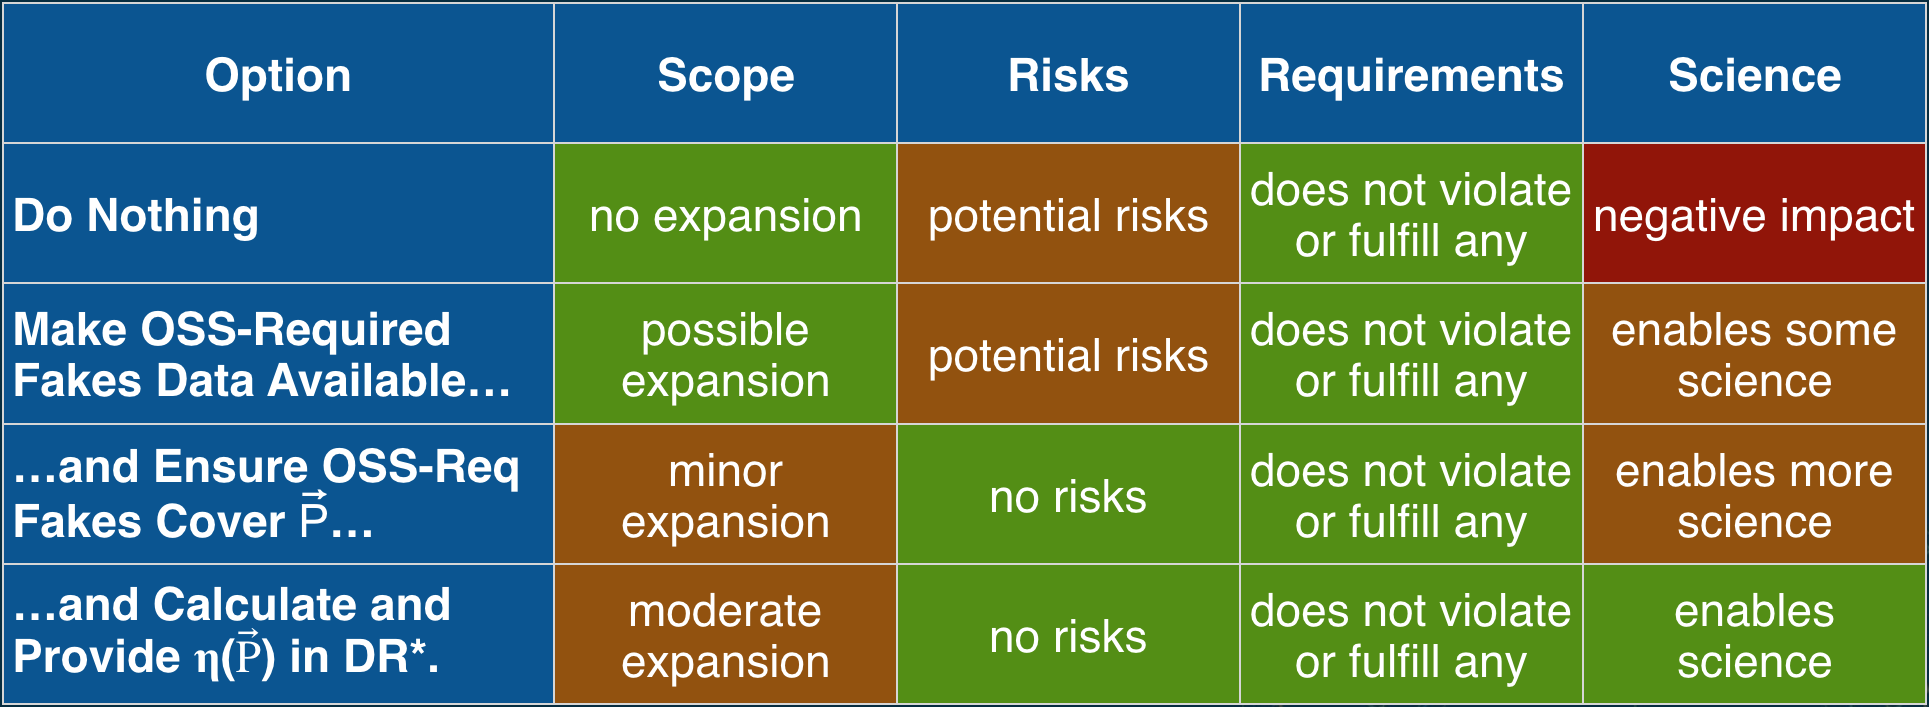
\includegraphics[width=15cm,trim={0cm 0cm 0cm 0cm}, clip]{figures/option_matrix.png}
\caption{A summary of the options with evaluated criteria, based on \S~\ref{sec:opts}. \label{fig:options}}
\end{center}
\end{figure}

This study is not yet finished and there remain some open questions to address, and further work is likely needed in order for an informed decision about the options proposed.

{\bf Open Questions for DM-SST:}\\
(1) Have DM's plans evolved away from what's in the documents (\S~\ref{sec:docs})? \\
(2) Does this work constitute a DMTN? It is not very technical -- yet. One option might be to take this to the TVS community for input and write a joint TVS-DM document, which incorporates the further study items below.

{\bf Further Study:}\\
 - establish the extent of the parameter space, $\vv{P}$\\
 - evaluate the accuracy needed for $\eta(\vv{P})$\\
 - does the mode of fake injection (\S~\ref{sec:opts}) matter for science?\\
 - will LSST's DIA be good enough to simply inject fakes into difference images?\\

\end{document}

